\begin{wrapfigure}{r}{60mm}
\vspace*{-7.8mm}
\begin{center}
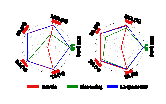
\includegraphics[width=60mm,height=!]{figs/Cifar_l1.pdf}

\vspace*{-1mm}
\begin{tabular}{cc}
{\scriptsize{\hspace*{-1.5mm}(a) Class-wise forgetting}} &{\scriptsize{\hspace*{3mm}(b) Random data forgetting}}
\end{tabular}
\end{center}
\vspace*{-2.5mm}


% 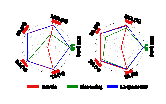
\includegraphics[width=60mm,height=!]{figs/Cifar_l1.pdf}}
% \vspace*{-2mm}
\caption{\footnotesize{
 Performance   of sparsity-aware unlearning vs. {\FT} and {\retrain} on class-wise forgetting and random data forgetting under (CIFAR-10, ResNet-18). 
 Each   metric is normalized to $[0,1]$ based on the best result  across unlearning methods 
  for ease of visualization, while the actual best value  is provided (\textit{e.g.}, $2.52$  is the  least computation time for class-wise forgetting). 
% \SL{[talk to me.]}
 % Each performance metric is normalized to $[0,1]$ 
 % using $1-\frac{|M-R|}{R}$, where $M$ denotes the different metrics from approximate unlearning, and $R$ denotes those from {\retrain}. {\RTE} is normalized to $[0,1]$ by using ${\frac{M}{\FT}}$. \JC{need to clarify that RTE is based on FT running time} \JH{updated}
% \JC{Merge to one figure and use one caption}
% \JC{Add `prune-first-then-unlearn'?}
}
}
%\JC{move other datasets (except cifar10) to appendix}
  \label{fig: results_l1_sparse_unlearn}
\vspace*{-7mm}
\end{wrapfigure}



% \begin{figure}[ht]
%     \centering
%     \begin{minipage}[htb]{75mm}
% \begin{center}
% \raisebox{-0.5cm}{ % Adjust this value as needed
% 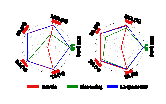
\includegraphics[width=0.95\textwidth,height=!]{figs/Cifar_l1.pdf}
% }

% \vspace*{-1mm}
% \begin{tabular}{cc}
% {\scriptsize{\hspace*{-1.5mm}(a) Class-wise forgetting}} &{\scriptsize{\hspace*{3mm}(b) Random data forgetting}}
% \end{tabular}
% \end{center}
% \vspace*{-2.5mm}
% \caption{\footnotesize{
%  Performance   of sparsity-aware unlearning vs. {\FT} and {\retrain} on class-wise forgetting and all-class random data forgetting under (CIFAR-10, ResNet-18). 
%  Each   metric is normalized to $[0,1]$ based on the best result  across unlearning methods 
%   for ease of visualization, while the actual best value  is provided (\textit{e.g.}, $2.52$  is the  least computation time for class-wise forgetting). 
% }
% }
%   \label{fig: results_l1_sparse_unlearn}
%     \end{minipage}
%     \hfill % To ensure that the figures are placed side by side
% \begin{minipage}[htb]{60mm}
% \begin{center}
%   \begin{tabular}{cccc}
%     \hspace*{-2mm}  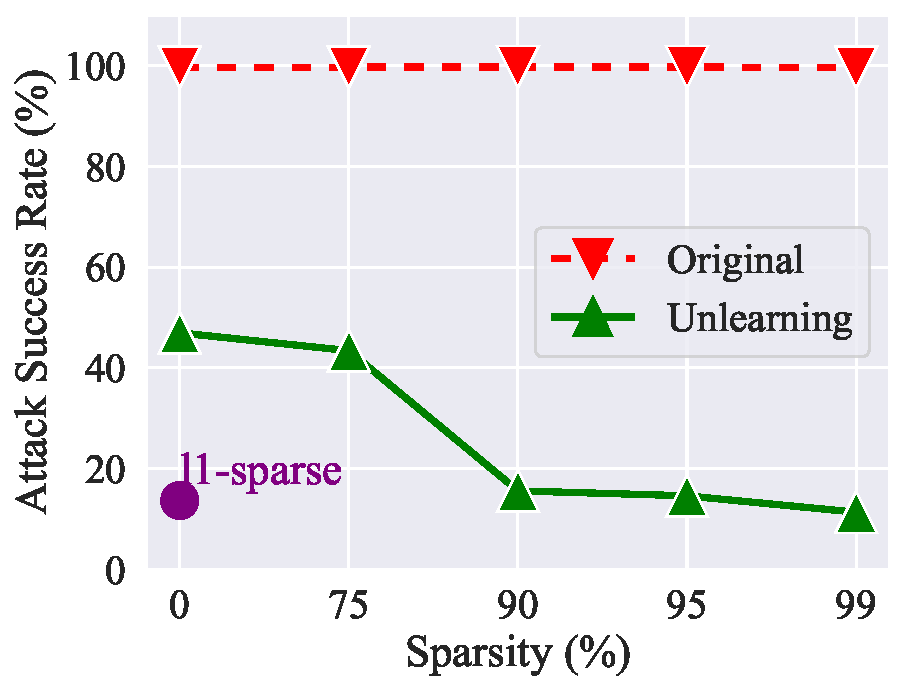
\includegraphics[width=30mm,height=!]{figs/rebuttal/backdoor_ASR.pdf} &
%     \hspace*{-5mm} 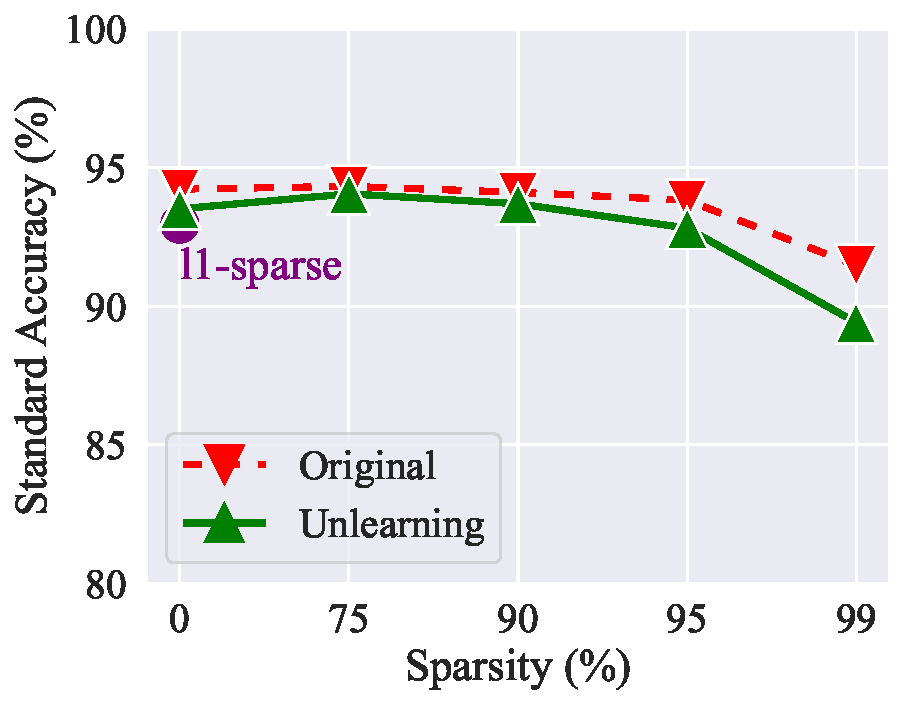
\includegraphics[width=30mm,height=!]{figs/rebuttal/backdoor_SA.pdf} \\
% \end{tabular}  
% \end{center}
% \vspace*{-2mm}
% \caption{
% % One figure demonstrates that our methods can decrease attack success rates and maintain good generalization performance.
% Performance  of  Trojan model cleanse   via proposed unlearning vs. model sparsity, where `Original' refers to the original Trojan model.
% %the effectiveness of the `Unlearn first, then prune' paradigm on the trojan model
% %cleanse application. 
% \textbf{Left}: ASR vs. model sparsity. \textbf{Right}: SA vs. model sparsity. 
% %Each marker represents the mean value over $10$ independent trials. %\JC{Add {\MUSparse}}
% %Results  The line and shaded area of each plot represent the mean and variance   over $10$ independent trials. 
% %\JC{remove variance}
% }
%   \label{fig: results_MU_pruning_backdoor}
%     \end{minipage}
% \end{figure}
